\documentclass{article}
\usepackage[utf8]{inputenc}
\usepackage{listings}
\usepackage{float}
\usepackage{algorithm}
\usepackage{fancyhdr}
\usepackage{xcolor}
\usepackage{graphics}
\usepackage{graphicx}

\begin{titlepage}
\title{\textbf{Network Lab Exam Question 3-B}}

\author{\\ \\  Albin Antony \\ Roll No:10 \\   TVE16CS010 }
\date{25 April 2019}

\end{titlepage}

\pagestyle{fancy}
\fancyhf{}
\rhead{Lab Exam}
\lhead{Que-3B}
\rfoot{\thepage}

\begin{document}
\definecolor{lightgray}{rgb}{.96,.96,.96}
\lstset{numbers=left, numberstyle=\tiny, stepnumber=1, numbersep=5pt,frame=hidden,breaklines=true,backgroundcolor=\color{lightgray},xleftmargin=0pt,xrightmargin=-20pt}
\pagenumbering{gobble}
  \maketitle
  \newpage
  \pagenumbering{arabic}
  \section{Calender Server}
  \subsection{Problem Statement}
 The idea is to create a calendar server based on TCP. You need to define a protocol (i.e.,
define how messages are formatted and transmitted), implement it, and write a client and a
server that communicate using your new connection-oriented protocol.
\newline
Your protocol should
support the following functionalities:
\begin{itemize}
\item1. Add a new calendar event.
\item2. Remove a calendar event.
\item3. Update an existing calendar event.
\item4. Get the events for a specific time or time range.
\end{itemize}

There are no other requirements regarding the protocol, i.e., you are free to decide the
protocol details, e.g., the message structure and content for the client/server communication.
  
  \subsection{Theory}
\subsubsection{TCP}
 TCP (Transmission Control Protocol) is a standard that defines how to establish and maintain a network conversation via which application programs can exchange data. TCP works with the Internet Protocol (IP), which defines how computers send packets of data to each other. Together, TCP and IP are the basic rules defining the Internet. TCP is defined by the Internet Engineering Task Force (IETF) in the Request for Comment (RFC) standards document number 793.
 \subsubsection{Client, Server and Socket}
 • Server-A server is a software that waits for client requests and serves or processes them accordingly.\newline
• Client- a client is requester of this service. A client program request for some resources to the server and server responds to that request.\newline
• Socket- Socket is the endpoint of a bidirectional communications channel between server and client. Sockets may communicate within a process, between processes on the same machine, or between processes on different machines. For any communication with a remote program, we have to connect through a socket port.

  \subsection{Algorithm}
%   algorithm file
  \begin{algorithm}[H]
  \lstinputlisting[language=c++]{algorithm/calserver}
  \caption{Algorithm for Server}
  \end{algorithm}
  The server receives arguments of client as a string from client.The string is split in a list.For add this list is appended to a calender list if does not exist in the list already. For deleting the calender list is searched to find the event if found it is removed.For update it is removed from calender list then the new venet is added.For get the event is searched based on the username and date, if found the even is send as response back to the client.\newline 
  
  For add, remove, update response is send as succes if not error occurs else a Duplicate entry error is sent.
  
  \begin{algorithm}[H]
  \lstinputlisting[language=c++]{algorithm/calclient}
  \caption{Algorithm for Client}
  \end{algorithm}
  
 \newpage

  \subsection{Program}
%   program file
\subsubsection{Server}
  \lstinputlisting[language=c++,numbers=none]{code/server.py}
  \newpage
  \subsubsection{Client}
  \lstinputlisting[language=c++,numbers=none]{code/client.py}
  \newpage
  \subsubsection{To run the program:}
   \begin{verbatim}

python server.py
python client.py hostname port [username] [action] [date] [time] [time] [Event]


  \end{verbatim}
  
  \subsection{Output}
\subsubsection{Test case 1}
 \begin{figure}[H]
\centering
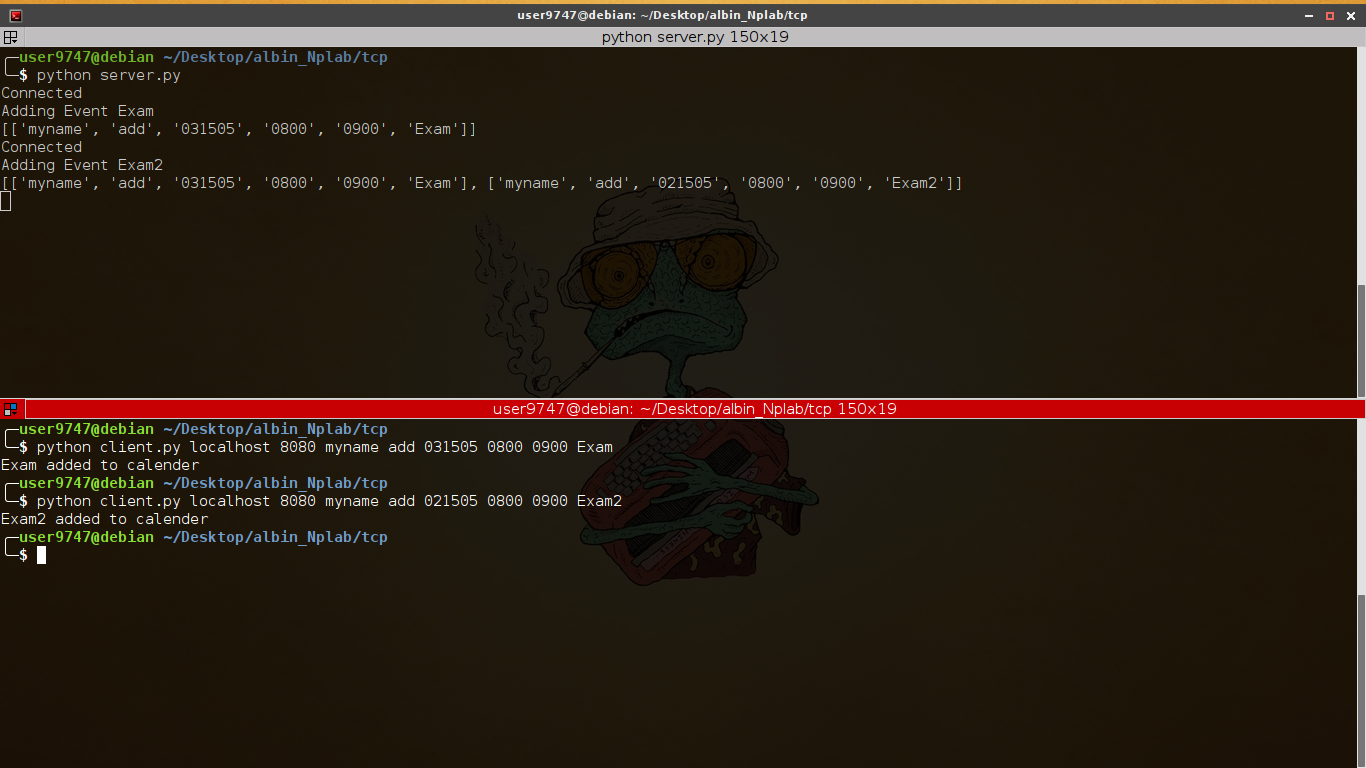
\includegraphics[width=400]{img/cal1.png}
\end{figure}

\subsubsection{Test case 2}
 \begin{figure}[H]
\centering
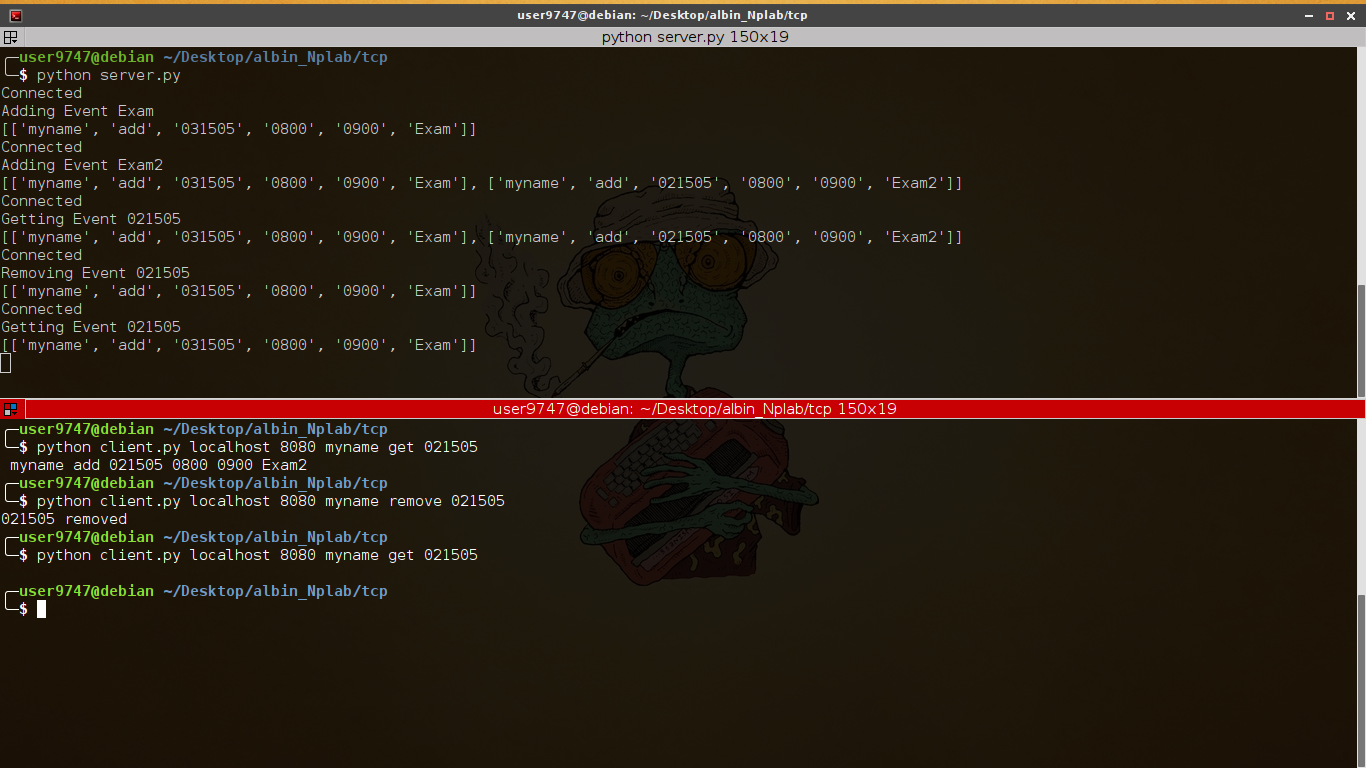
\includegraphics[width=400]{img/cal2.png}
\end{figure}

\subsubsection{Test case 3}
 \begin{figure}[H]
\centering
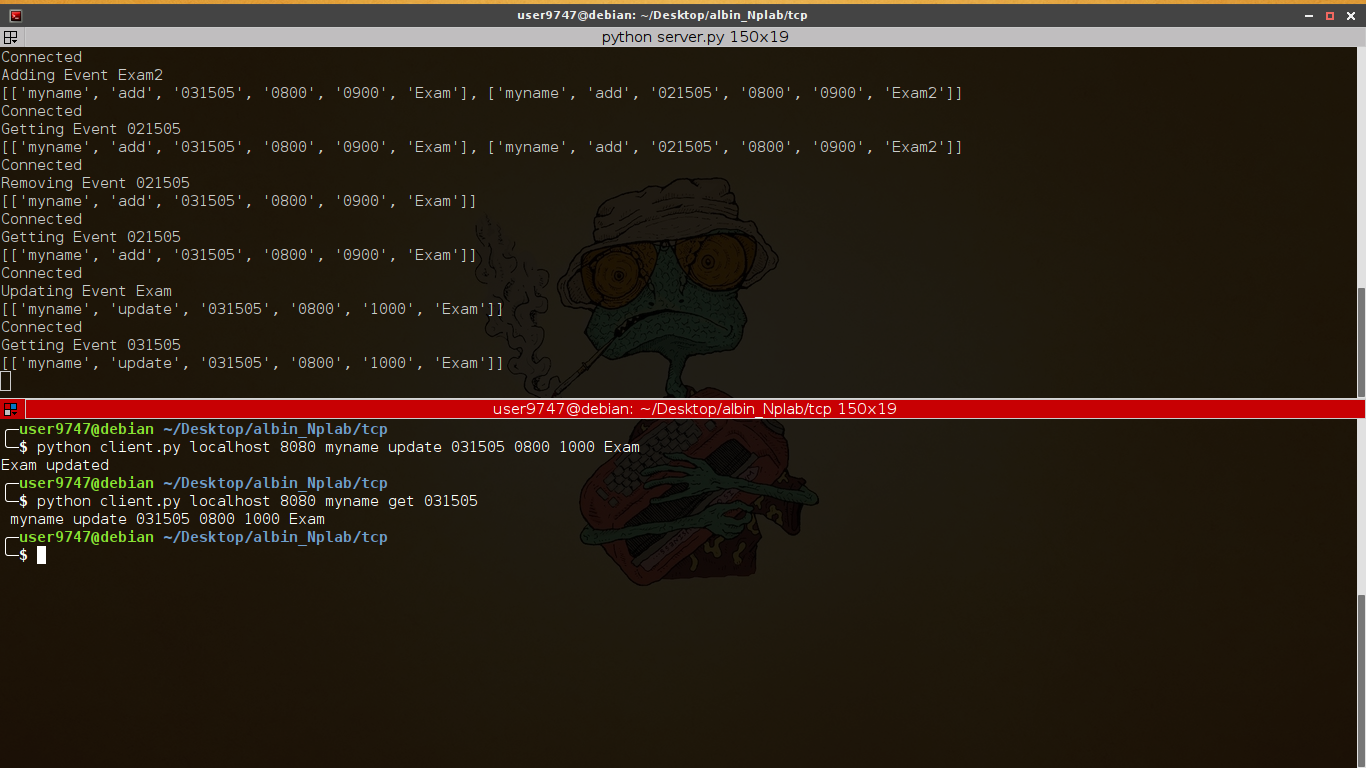
\includegraphics[width=400]{img/cal3.png}
\end{figure}
  
  
  

\end{document}